
CLAS12 acceptances and resolutions are also superior to that of CLAS6. Main differences are:
- RGK has outbending torus vs inbending CLAS6 data
- the distance between the target and the PCal has increased, the FTCal extends to lower angles, and the gap between FTCal and PCal is much smaller than between IC and EC
- proton polar angle was limited to 60 deg in the e1dvcs dataset if my memory is correct


    volker clas12 exp \cite{Burkert2020TheLaboratory}


    in beam dump area, link to own fraday cup paper \cite{Johnston2019RealizationElectrons}
    \begin{figure}[H]
        \centering
        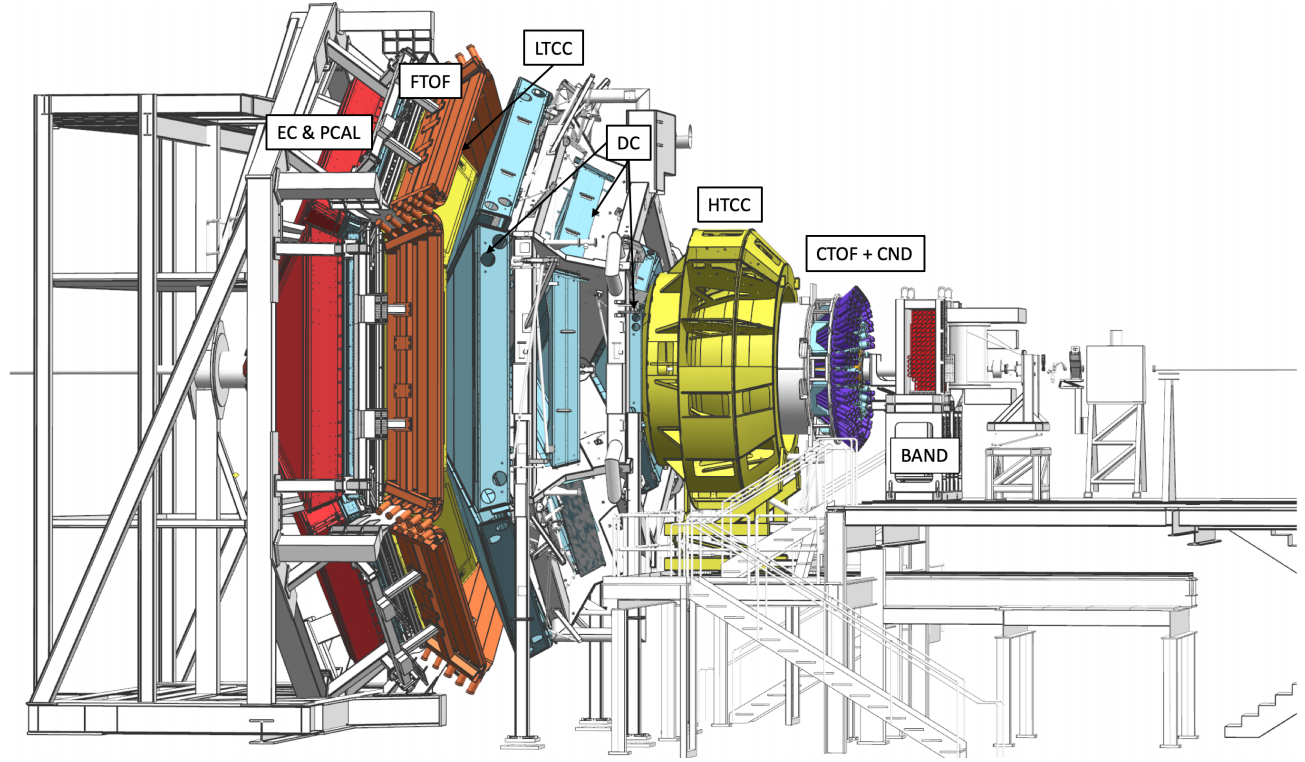
\includegraphics[width=12cm]{Chapters/Ch2-Experiment/clas-12-system/pics/other/CLA12.PNG}
        \caption{ CLAS12 Detector System }
    \end{figure}
    
    \begin{figure}[H]
        \centering
        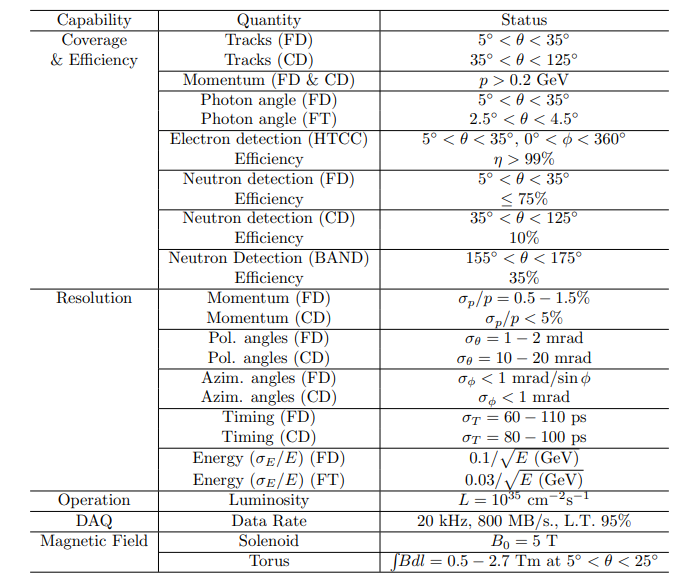
\includegraphics[width=10cm]{Chapters/Ch2-Experiment/clas-12-system/pics/other/clas12-params.PNG}
        \caption{CLAS12 Specification}
    \end{figure}

    \begin{figure}[H]
        \centering
        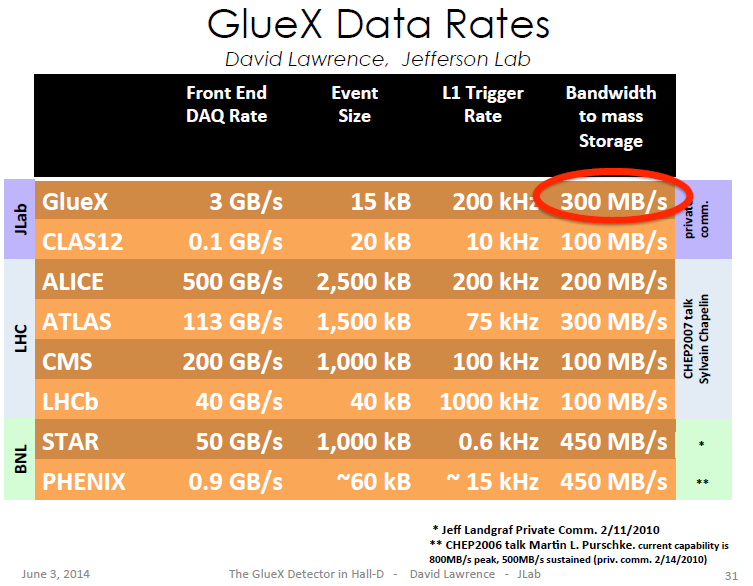
\includegraphics[width=10cm]{Chapters/Ch2-Experiment/clas-12-system/pics/other/good_data_rates_slide.PNG}
        \caption{CLAS12 Data Rates, Compared to Other Experiments }
    \end{figure}

    
        \subsection{Thomas Jefferson National Accelerator Facility}
            \subsubsection{Electron Source}    
            \subsubsection{Polarimeters}
                    As stated, for RGA, the fact that the beam is polarized is not useful, but it is true and is measured by Moller Polarimeters. 
    
           
    
            Polarimietry: 
                    Good for beam energies between 100 MeV and 50 GeV. Polarized beam electrons are scat-
            tered from other polarized electrons in a target, usually magnetized foils. Only a small
            fraction of all the target electrons are polarized, so this method has a small analyzing
            power. Analyzing power is exactly calculable in QED. At high beam energies, analyzing
            power and scattering probability both become independently of beam energy. Maximum
            analyzing power is about 80%, maximum is at 90 degrees scattering angle in C.o.M. Trans-
            versely polarized target can be used to measure transverse beam polarization, but analyzing
            power is only about 10%. 90 degrees C.o.M. translates to a small lab angle with each elec-
            tron at half beam energy, so magnets are used to bend these electrons out to detectors.
            These detectors can be, for example lead glass total absorption cherenkov counters.Since
            the two electrons are corellated, can use things like time coincidence to reduce background,
            although for low duty factor accelerators only one electron is required as statistics would
            otherwise be too low.A main background to this process is Mott scattering with the electron
            radiating off energy after scattering, appearing as a Moller electron
            
            The scattering target is either iron or vanadium permendur (iron-cobalt alloy). Only 2 of
            26 electrons in iron have their spins oriented, leading to a total analyzing power of only 6 percent
            and transverse analyzing power of only 1%. Uncertainties in how magnetized the targets
            actually are corresponds to an uncertainty in analyzing power. There are ’easy’ and ’hard’
            magnetization schemes - easy does a soft magnetization, while hard uses a several tesla mag-
            net to saturate the target. In principle, uncertainties on magnetization in the hard scheme
            can be removed by using the Kerr magneto-optic effect, but this has not ever been imple-
            mented. An important correction is due to the Levchuk effect, where due to momentum
            differences between electrons in different shells, electrons scattered off of polarized electrons
            are more likely to be detected than off of unpolarized electrons. Specifically, inner electrons
            are unpolarized and have a large average momenta, so when struck they can fall outside the
            113 TOC
            acceptance of the Moller detectors, while the outer electrons, which are polarized, have a
            small average momentum, and behave as expected. This is up to a 15% effect on polarization
            measurements, and is currently a work in progress.
            
            \subsubsection{Accelerator}
                    For entry into CLAS12, the beamline specs are as follows:\\
                    Beam current: up to 50 nA\\
                    Beam energy spread: $10^-4$\\
                    Beam size: Less than 0.4 mm\\
                    Beam stability: Less than 0.1 mm\\
                    Beam halo: $10^-4$\\
                    Beam polarization: up to 80\%\\
    
    
            
        \subsection{CLAS12 Beamline}
            \subsubsection{Liquid Hydrogen Target}
                Rasterization of some kind
                \\
                \indent The hydrogen target in RGA is cooled to 20 K using a He4 evaporation fridge. Can by polarized by dynamic nuclear polarization, driven by a 140 GHz microwave source, can reach 90\% polarization for protons, 40\% for deuterons (both longitudinally polarized). The polarization can be measured by a Q-meter based NMR. 2.5 cm diameter target, extended 5 cm long. \\
                \indent RGA does not use a polarized target. The beam is polarized, but the target is not, so polarization is not helpful for extracting the 5-fold differential cross section (but it would be if the target was also polarized, and is useful for BSA measurements).
            
            \subsubsection{Faraday Cup and Beam Dump}
            Luminosity in CLAS12 is measured from the Faraday Cup and using reference reactions such as elastic scattering. We don't use the Faraday Cup event by event, but we do use it run by run. For beam current measurements, beam position monitors upstream are used - but this is for monitoring on-line, not for analysis.
                       Can manage 175 Watts - 17 nA at 10 GeV. Is used to calibrate beam current, needs a blocker in at higher currents.